\documentclass{article}
\usepackage{graphicx}
\usepackage{blindtext}
\usepackage[top=1.5in,bottom=1.5in,left=1.75in,right=1.75in]{geometry}
\begin{document}
\begin{center}
\set{linewidth=2.0in}
\includegraphics[width=.5\linewidth]{1.png}\quad\includegraphics[width=.5\linewidth]{1_cos.png}
\\
\includegraphics[width=.3\linewidth]{1_3d.png}\quad\includegraphics[width=.3\linewidth]{1_cos_3d.png}
\\
\includegraphics[width=.3\linewidth]{2.png}\quad\includegraphics[width=.3\linewidth]{2_cos.png}
\\
\includegraphics[width=.3\linewidth]{2_3d.png}\quad\includegraphics[width=.3\linewidth]{2_cos_3d.png}
\\
\includegraphics[width=.3\linewidth]{3.png}\quad\includegraphics[width=.3\linewidth]{3_cos.png}
\\
\includegraphics[width=.3\linewidth]{3_3d.png}\quad\includegraphics[width=.3\linewidth]{3_cos_3d.png}
\\
\includegraphics[width=.3\linewidth]{4.png}\quad\includegraphics[width=.3\linewidth]{4_cos.png}
\\
\includegraphics[width=.3\linewidth]{4_3d.png}\quad\includegraphics[width=.3\linewidth]{4_cos_3d.png}
\\
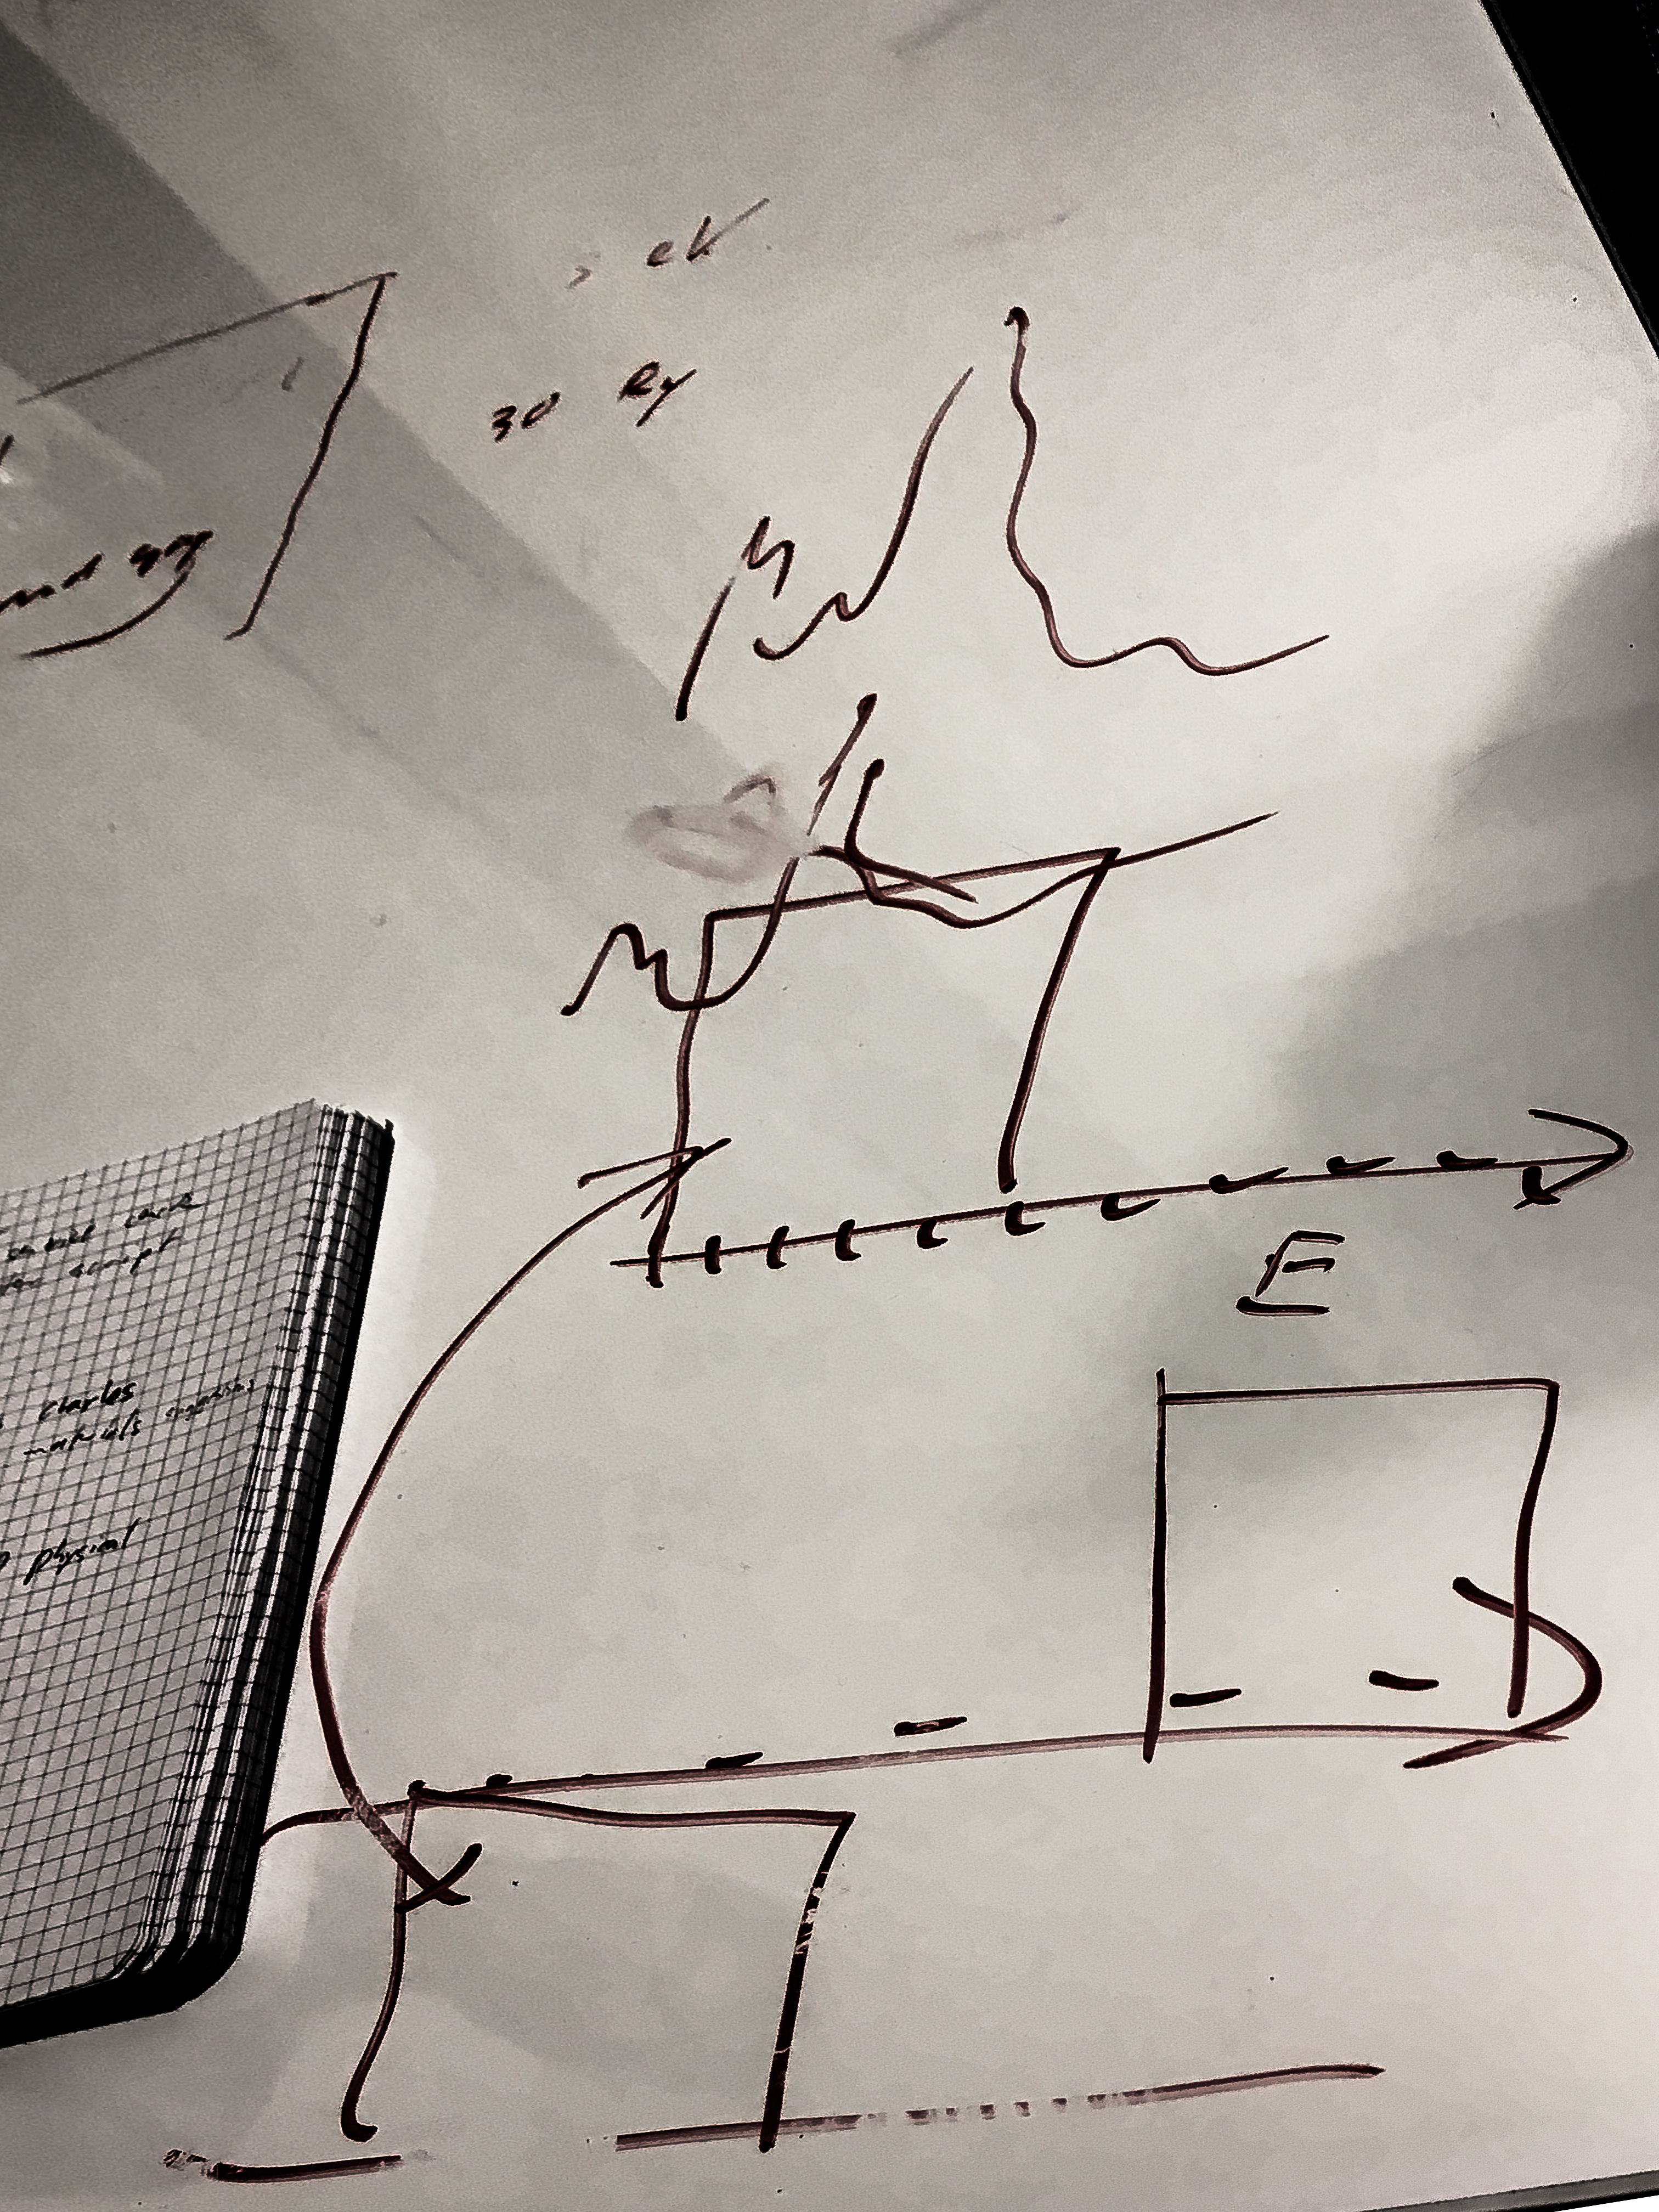
\includegraphics[width=.3\linewidth]{5.png}\quad\includegraphics[width=.3\linewidth]{5_cos.png}
\\
\includegraphics[width=.3\linewidth]{5_3d.png}\quad\includegraphics[width=.3\linewidth]{5_cos_3d.png}
\end{center}
\end{document}

